%Correct the file name.
%X: book number
%Y: part number
%ZZZ: page number in three digits. So page 3 would be 003.

\documentclass[11pt]{amsbook}

\usepackage{../HBSuerDemir}	% ------------------------


\begin{document}

% ++++++++++++++++++++++++++++++++++++++
\hPage{b2p1/259}
% ++++++++++++++++++++++++++++++++++++++
	\begin{enumerate}
		\item[199.]
			Find the locus of the point ratio of its distance from the point $A(2, 0, 0)$ and the plane $\pi : x = 1$ is 2.

    	\item[200.]
    		Find the locus of the points, ratio of its distances from the point $A(0, 0, 2)$ and $B(0, 0, -2)$ is 3.

    	\item[201.]
    		Find the equation of the planes whose intersection with the ellipsoid $9x^2 + 25y^2 + 169z^2 = 1$ are circles.
    	
		\item[202.]
			Find the condition that $(x_1, y_1, z_1)$ should be the middle point of the chord of the hyperholoid $x^2 - y^2 + 4z^2 = 16$ formed by \\
			$\frac{x-x_1}{2} = \frac{y-y_1}{-1} = \frac{z-z_1}{-2}$

    	\item[203.]
    		Find the condition that the line $\frac{x-2}{\cos \alpha} = \frac{y-1}{\cos \beta} = \frac{z+1}{\cos \gamma}$ should be tangent to the paraboloid $x^2-y^2+3z = 0$.

		\item[204.]
			Let $\vec{P} = (\cos \lambda t)A + (\sin t)B$ where $\lambda$, A, B are constant. Show that\\
			a)$P \times \frac{dP}{dt} = Const$
			b)$\frac{d^2 P}{dt^2} + \lambda^2 P = 0$

		\item[205.]
			If $P(t), Q(t)$ are vector functions, show that\\
			a)$\frac{d}{dt}(P \times \frac{dP}{dt}) = P \times \frac{d^2p}{dt^2}$
			b)$P \cdot \frac{dP}{dt} = |P| \frac{d}{dt}|P|$\\
			c)$|\frac{dP}{dt}| = \frac{d}{dt}|P|$
			d)$\frac{d}{dt} (P \times \frac{dQ}{dt} - \frac{dP}{dt} \times Q) = P \times \frac{d^2 Q}{dt^2} - \frac{d^2p}{dt^2} \times Q$

		\item[206.]
			Let P, Q be two fixed points of a solid in motion, and let $\vec{V}(P), \vec{V}(Q)$ be the velocity vectors at P and Q. Show that the projections of these velocitions on the line PQ are equal to each other.

		\item[207.]
			Find the arc length of the VIVIANI curve $\Gamma : x^2 + y^2 + z^2 = 4a^2$ , $x^2 + y^2 - 2ax = 0$ in the first octant.
		
	\end{enumerate}
\end{document}  

%==== templates ====

%==== environments ====

%\begin{figure}[htb]
%	\centering
%	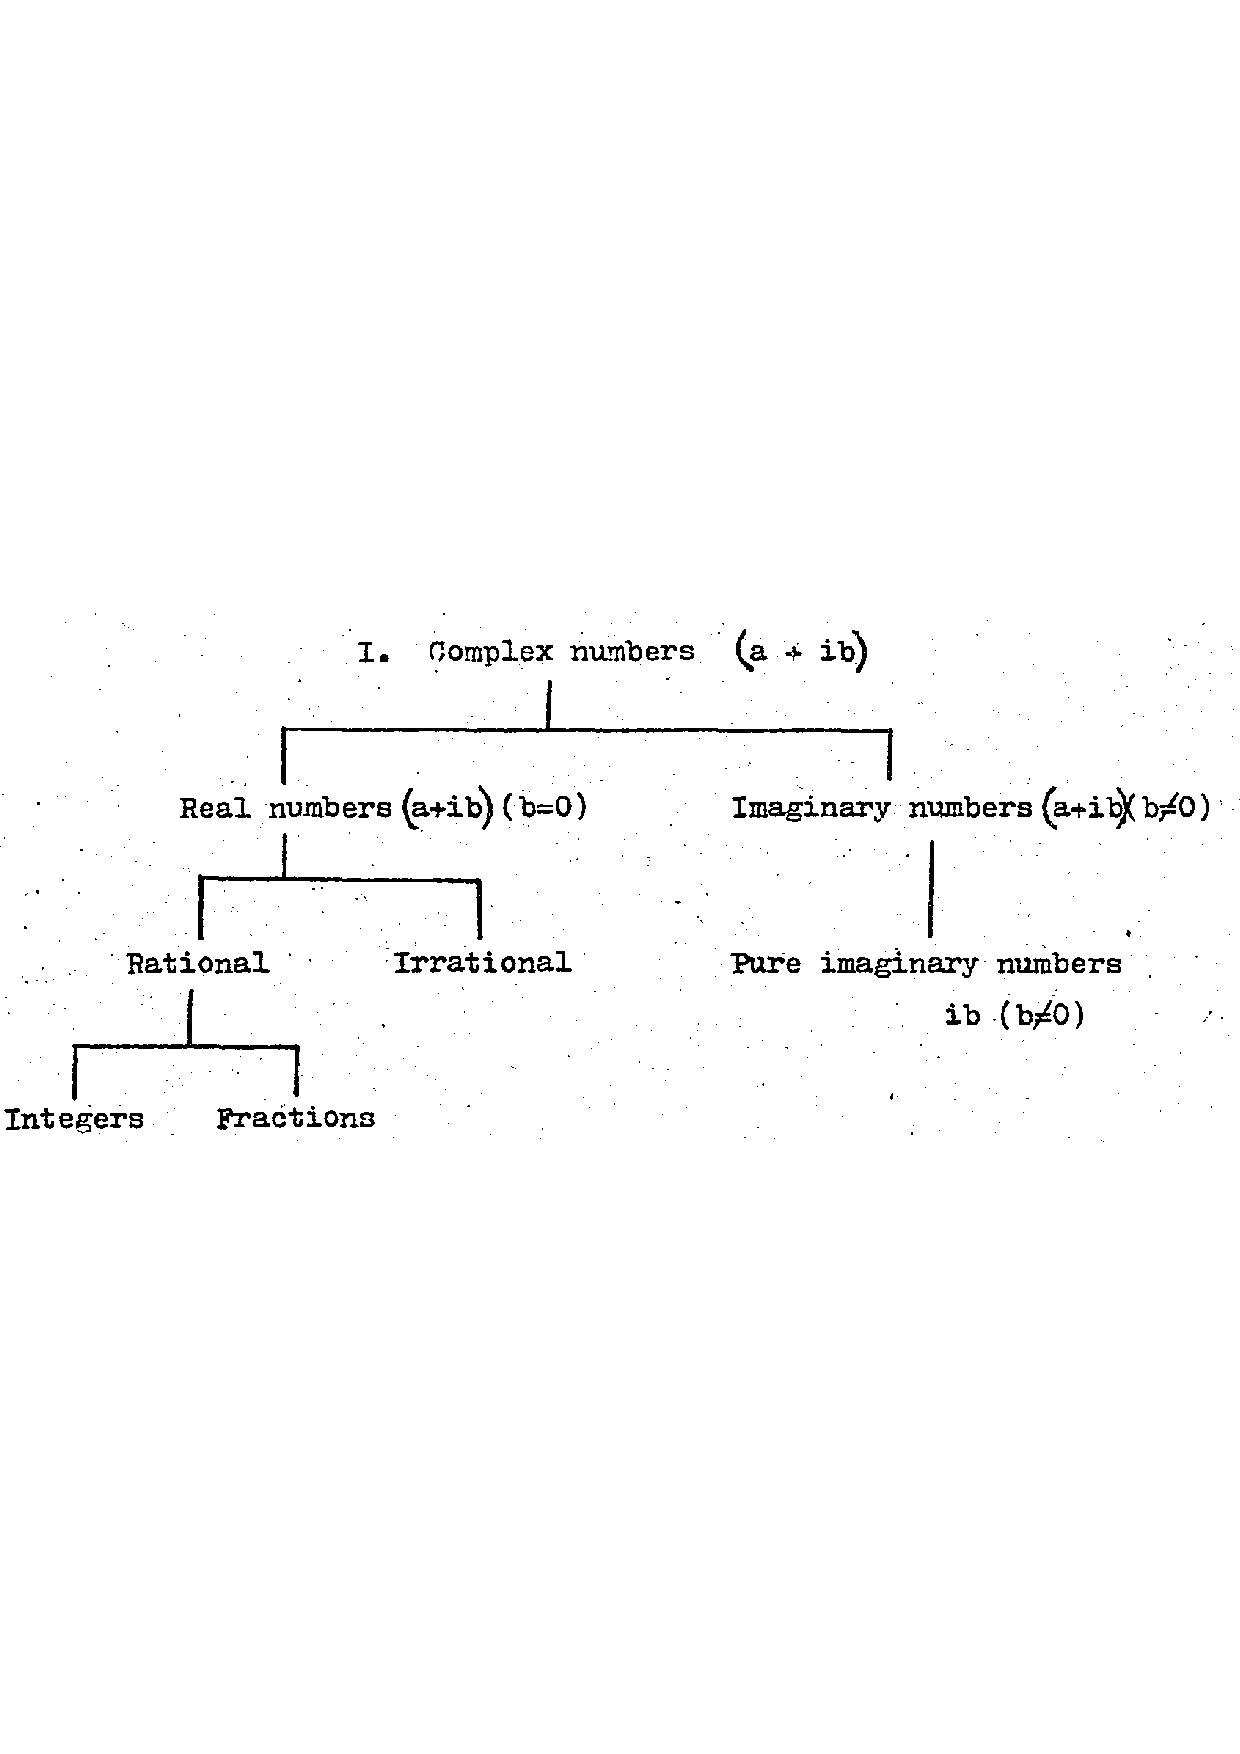
\includegraphics[width=0.9\textwidth]{images/SD-1-1p15A}
%	\caption{Classification of complex numbers}
%	\label{fig:classificationOfComplexNumbersA}
%\end{figure}

%\begin{center}
%\begin{tabular}{cc}
%\end{tabular}
%\end{center}

%\begin{exmp}
%\begin{hSolution}
%\end{hSolution}
%\end{exmp}

%\begin{hEnumerateAlpha}
%\end{hEnumerateAlpha}

%\begin{hEnumerateRoman}
%\end{hEnumerateRoman}

%$
%\begin{bmatrix}
%\end{bmatrix}
%$

%\frac{aaaa}{bbb}
%\frac{a_{n}}{b_{n}}
%\left( aaaa \right)
%\Longrightarrow

%\begin{multicols}{2}
%	bb
%\columnbreak
%	aa
%\end{multicols}
